% !TeX document-id = {9ccc6fb7-c5f4-4308-9c17-4c226ad62230}
%%%%%%
%
% $Autor: Alpizar, Kumari, JK $
% $Datum: 2023-01-31 11:59:00Z $
% $Version: 1.0.0 $
%
%
% !TeX encoding = utf8
% !TeX root = Rename
% !TeX TXS-program:bibliography = txs:///biber
%
%%%%%%

\chapter{Knowledge Discovery in Databases Process}

The basic definition of KDD in \autocite{Fayyad:1996} describes it as a nontrivial process of "identifying valid, novel, potentially
useful, and ultimately understandable patterns in data". \autocite{Fayyad:1996} mentions that in the context of KDD, description tends to be more important than prediction. The paper also lists the detailed steps of KDD process as mentioned below:

\begin{enumerate}
	\item Developing an understanding of the application domain and the relevant prior knowledge.
	\item Selecting the target data set on which discovery is to be performed
	\item Cleaning and pre processing the data to handle noise and missing data fields
	\item Find useful features to represent the  data depending on the goal of
	the task. Thenafter, use transformation methods to find more suitable representation for the data.
	\item Identify appropriate methods to search for patterns in data as part of data mining.
	\item Interpreting and evalutaing the results from data mining. This step
	can also involve data visualization of the extracted patterns/models.
	\item The final step is to consolidate discovered knowledge and share with another system or report to interested parties.
	\item Even after the completion of the final step we need to monitor the performance after the addition of new data and recheck the results.
\end{enumerate}

The above steps can be summarised using figure \ref{fig:KDDprocess}  : 

\begin{figure}  [H]
	\begin{center}
		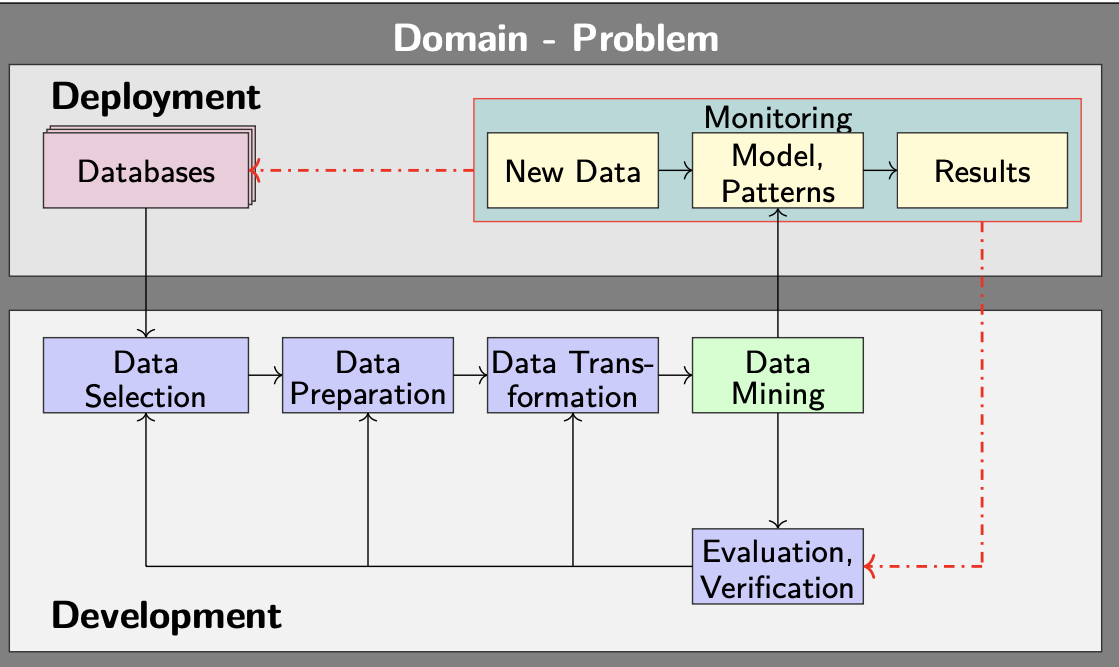
\includegraphics[width=10cm]{KDDprocess}
		\caption{KDD process} \label{fig:KDDprocess}
		%{\footnotesize \textbf{Reference:} \autocite{Network2020}}
	\end{center}
\end{figure}

The detailed description of how we acheived each individual step will be described in next chapter.

